Another pattern that the researchers noticed is between the composers of the Barque, Classical and 19th Century. A unique pattern was observed to these two Baroque composers Boyce and Sammartini. Both composers have the most similar pattern in the Baroque Period as shown below.

\begin{figure}[!htb]
\begin{minipage}{.5\textwidth}
  \captionof{figure}{Baroque: Boyce}
  \centering
  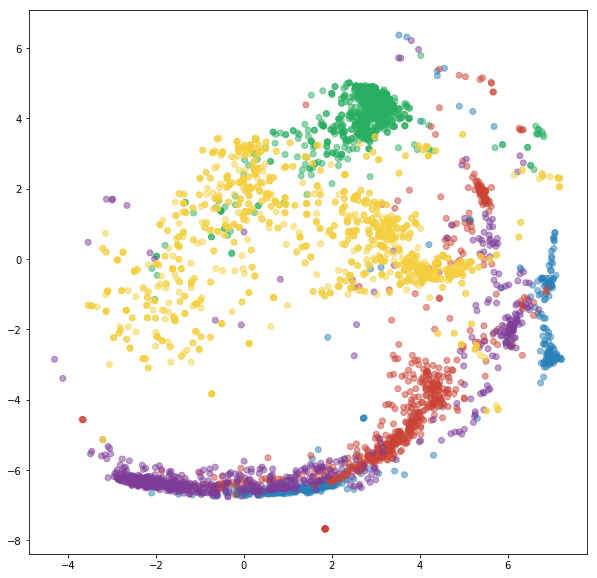
\includegraphics[scale=0.15]{P1C2}
  \label{fig:test2}
\end{minipage}
\begin{minipage}{.5\textwidth}
  \captionof{figure}{Baroque: Sammartini}
  \centering
  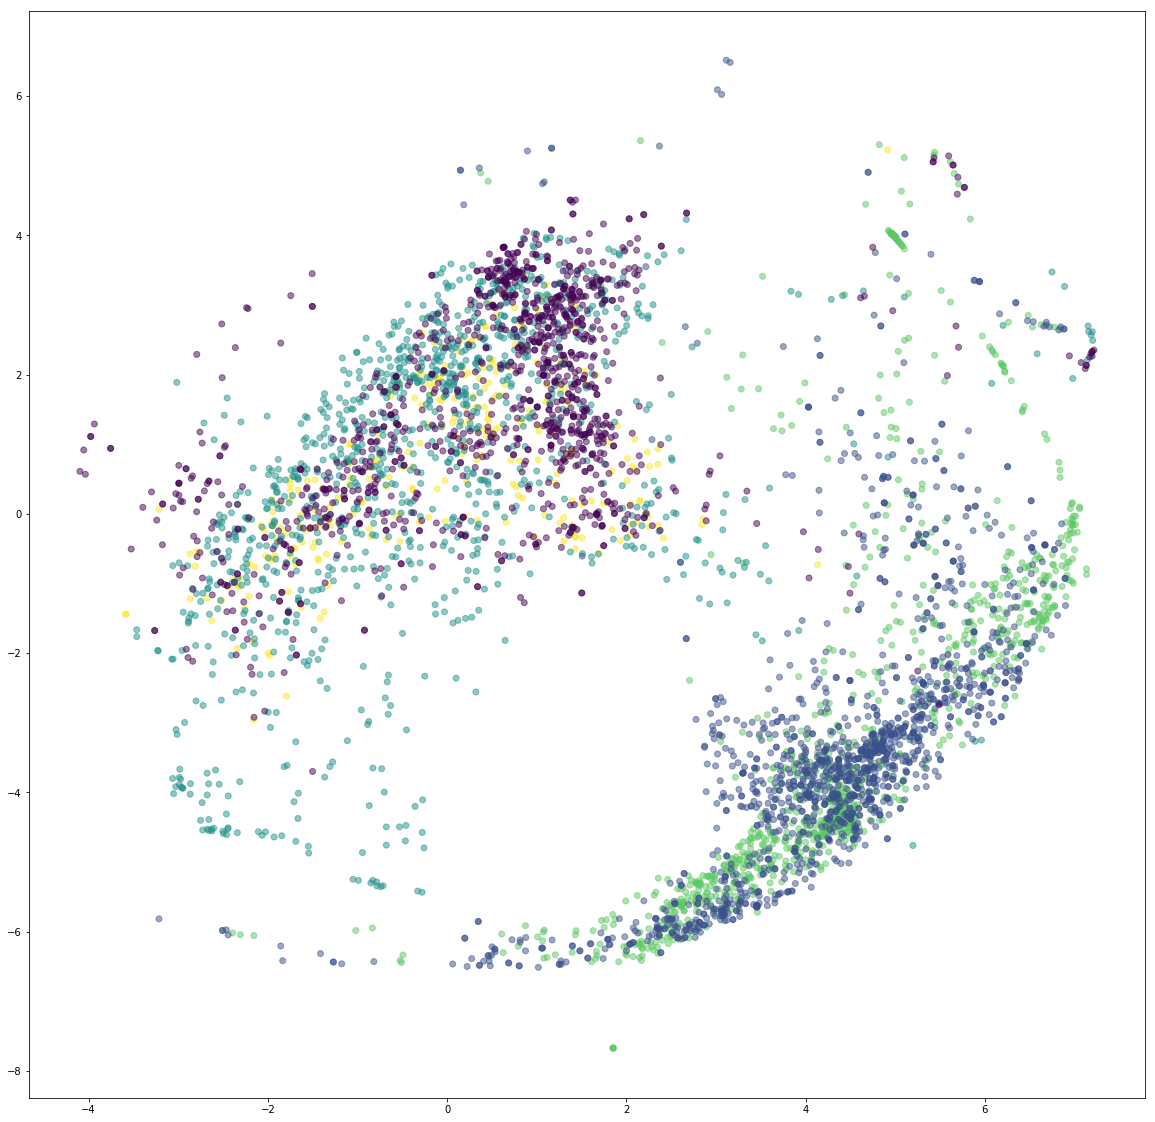
\includegraphics[scale=0.15]{P1C4}
  \label{fig:test2}
\end{minipage}
\end{figure}

In the Classical Period, composer Haydn had the same pattern except on the top left part of the graph. The research considered that the pattern of Haydn is still relevant or influenced by the Baroque composers because the left and bottom part of the graph is similar. Two of Haydn’s are the ones that influence the change of the graph in comparison to the Baroque composers. The graphs of the said composers would be more similar without the two works of Haydn. Moving on to the Classical period, the trends was observe to be present in the works of Clementi. Just like Haydn’s, the same top left area is the main difference compared to the Baroque composers that was also caused by two of his compositions. Without the blue and yellow points of Clementi, the graph would become more similar with the other composers.

\begin{figure}[!htb]
\begin{minipage}{.5\textwidth}
  \captionof{figure}{Classical: Haydn}
  \centering
  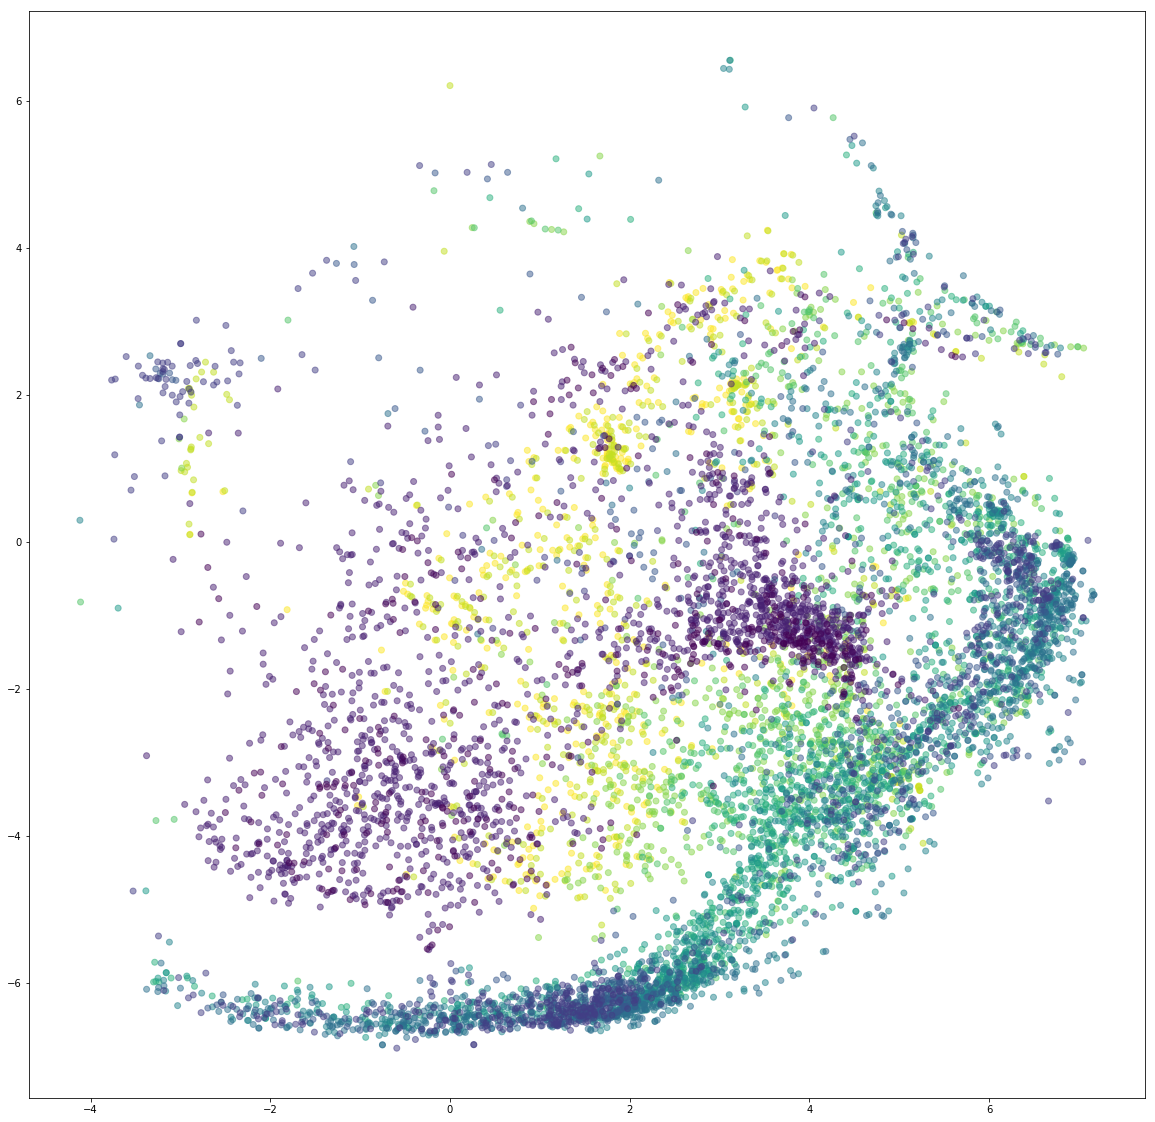
\includegraphics[scale=0.15]{P2C3}
  \label{fig:test1}
\end{minipage}
\begin{minipage}{.5\textwidth}
  \captionof{figure}{19th Century: Clementi}
  \centering
  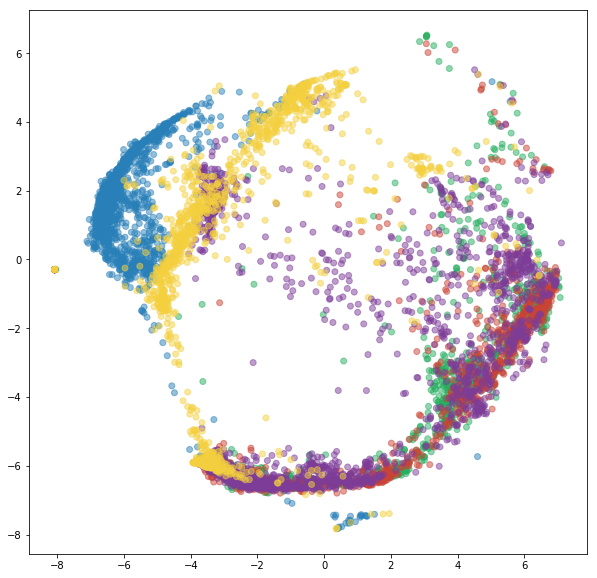
\includegraphics[scale=0.15]{P3C2}
  \label{fig:test2}
\end{minipage}
\end{figure}

Lastly, the same pattern extended until the 20th Century with composer Stravinsky. Stravinsky has a very similar pattern with the 19th Century composers. Shown below is the graph of Stravinsky.

\begin{figure}[!htb]
\caption{20th Cen: Stravinsky}
\centering
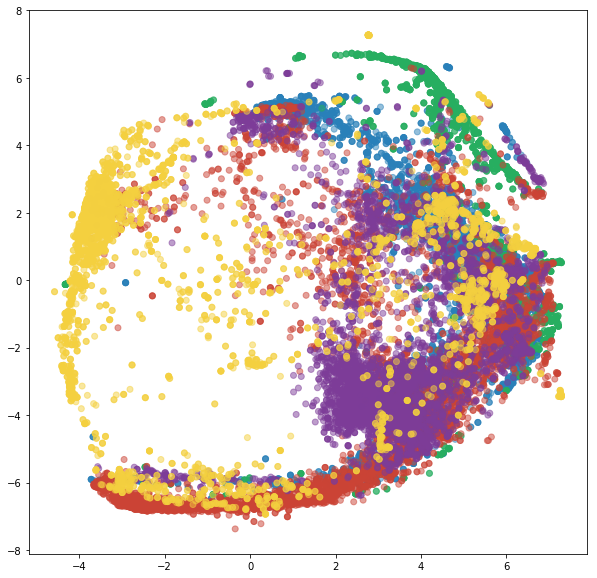
\includegraphics[scale=0.15]{P5C5}
\end{figure}

The results of the graphs may suggest that the works of the 19th and 20th Century composers are influenced by previous periods. The works of Boyce and Sammartini are the root of this specific style pattern that might be adapted to the next period. 

The researchers also noticed a pair of composers which had the most distinguishable pattern because the points are only located in the left side of the graph. 19th Century composer Gossec and 20th Century composer Antheil produced similar style pattern which may suggest that Antheil’s work is influenced by Gossec.

\begin{figure}[!htb]
\begin{minipage}{.5\textwidth}
  \captionof{figure}{19th Century: Gossec}
  \centering
  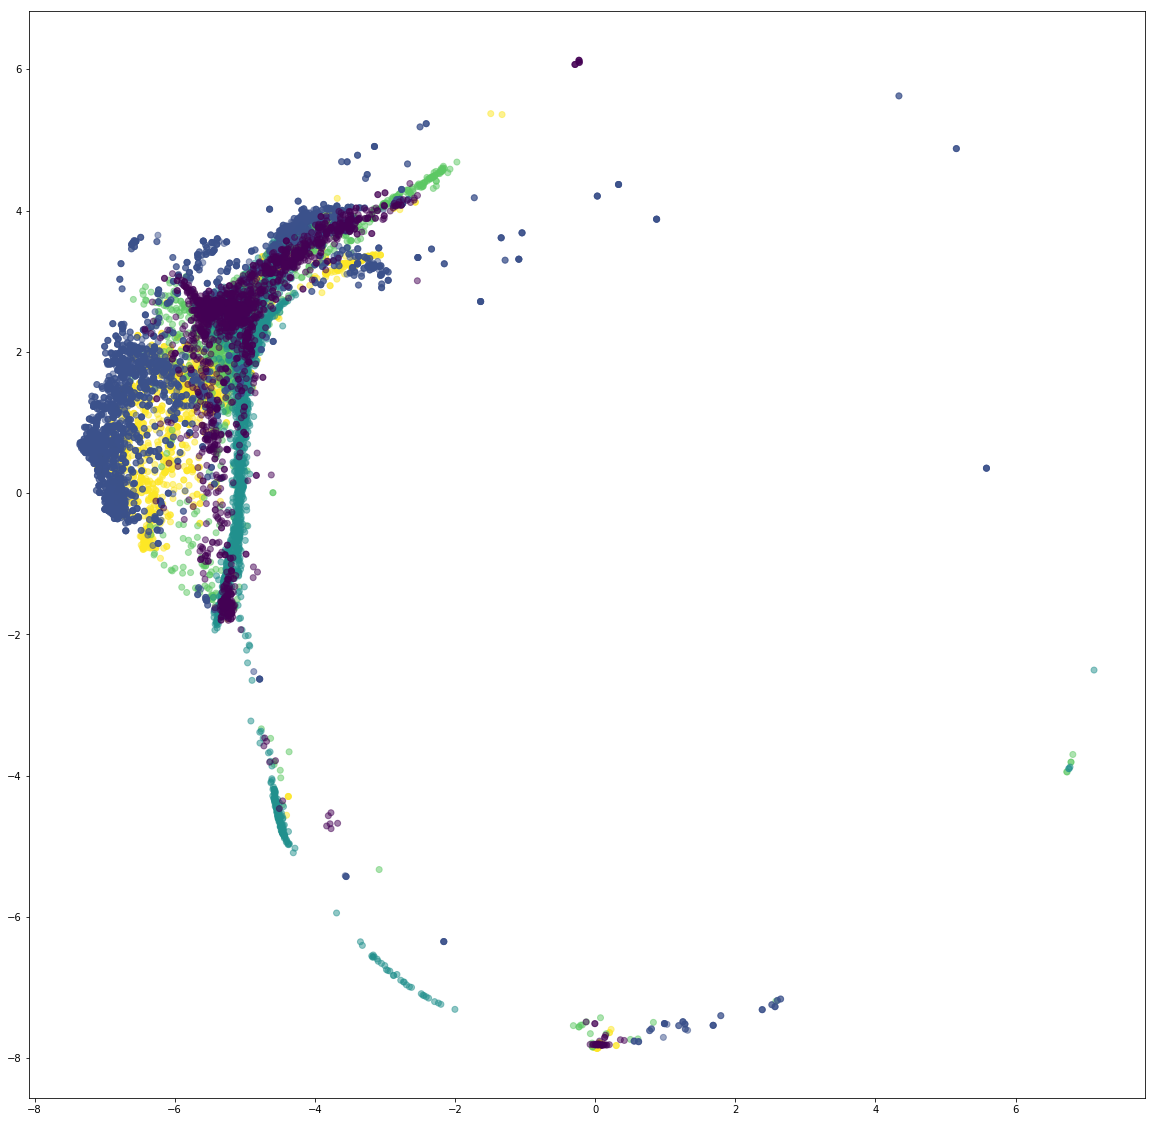
\includegraphics[scale=0.15]{P3C3}
  \label{fig:test1}
\end{minipage}
\begin{minipage}{.5\textwidth}
  \captionof{figure}{20th Cen: Antheil}
  \centering
  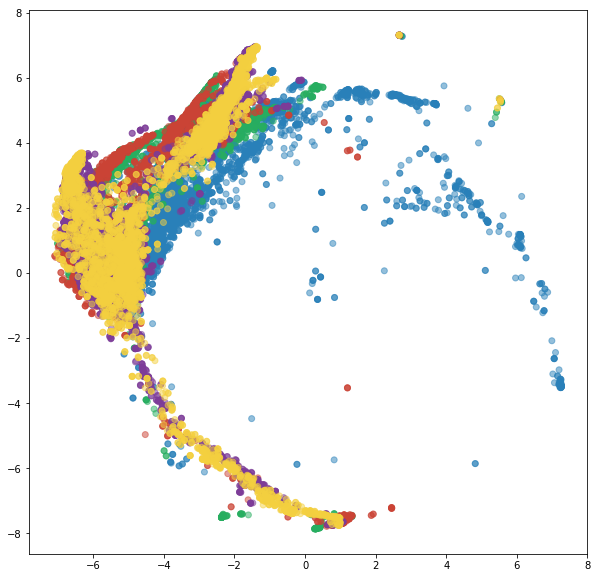
\includegraphics[scale=0.15]{P5C1}
  \label{fig:test1}
\end{minipage}
\end{figure}